\section{Conclusions}


\section{Future Work}

The results of this work show that a system is able to autonomisly learn to handover objects and adapt to novel ones, but some caveats do exist for it to become truly autonomous. The largest problem is object detection, which is a challenging field within computer vision. This work took help of AprilTags to locate and track the objects but in a live environment these tags do not exist on all objects and the system would need a better way of recognizing the object in the handover scene to extract data about the handover. Some work show good success using alternatives such as point cloud libraries (\parencite{Chan2015a}). Object detection using point clouds was tried in this work before using AprilTags, but with very poor results. This is something that would need more work to try and implement better without the help of the tags.

\begin{figure}
	\centering
	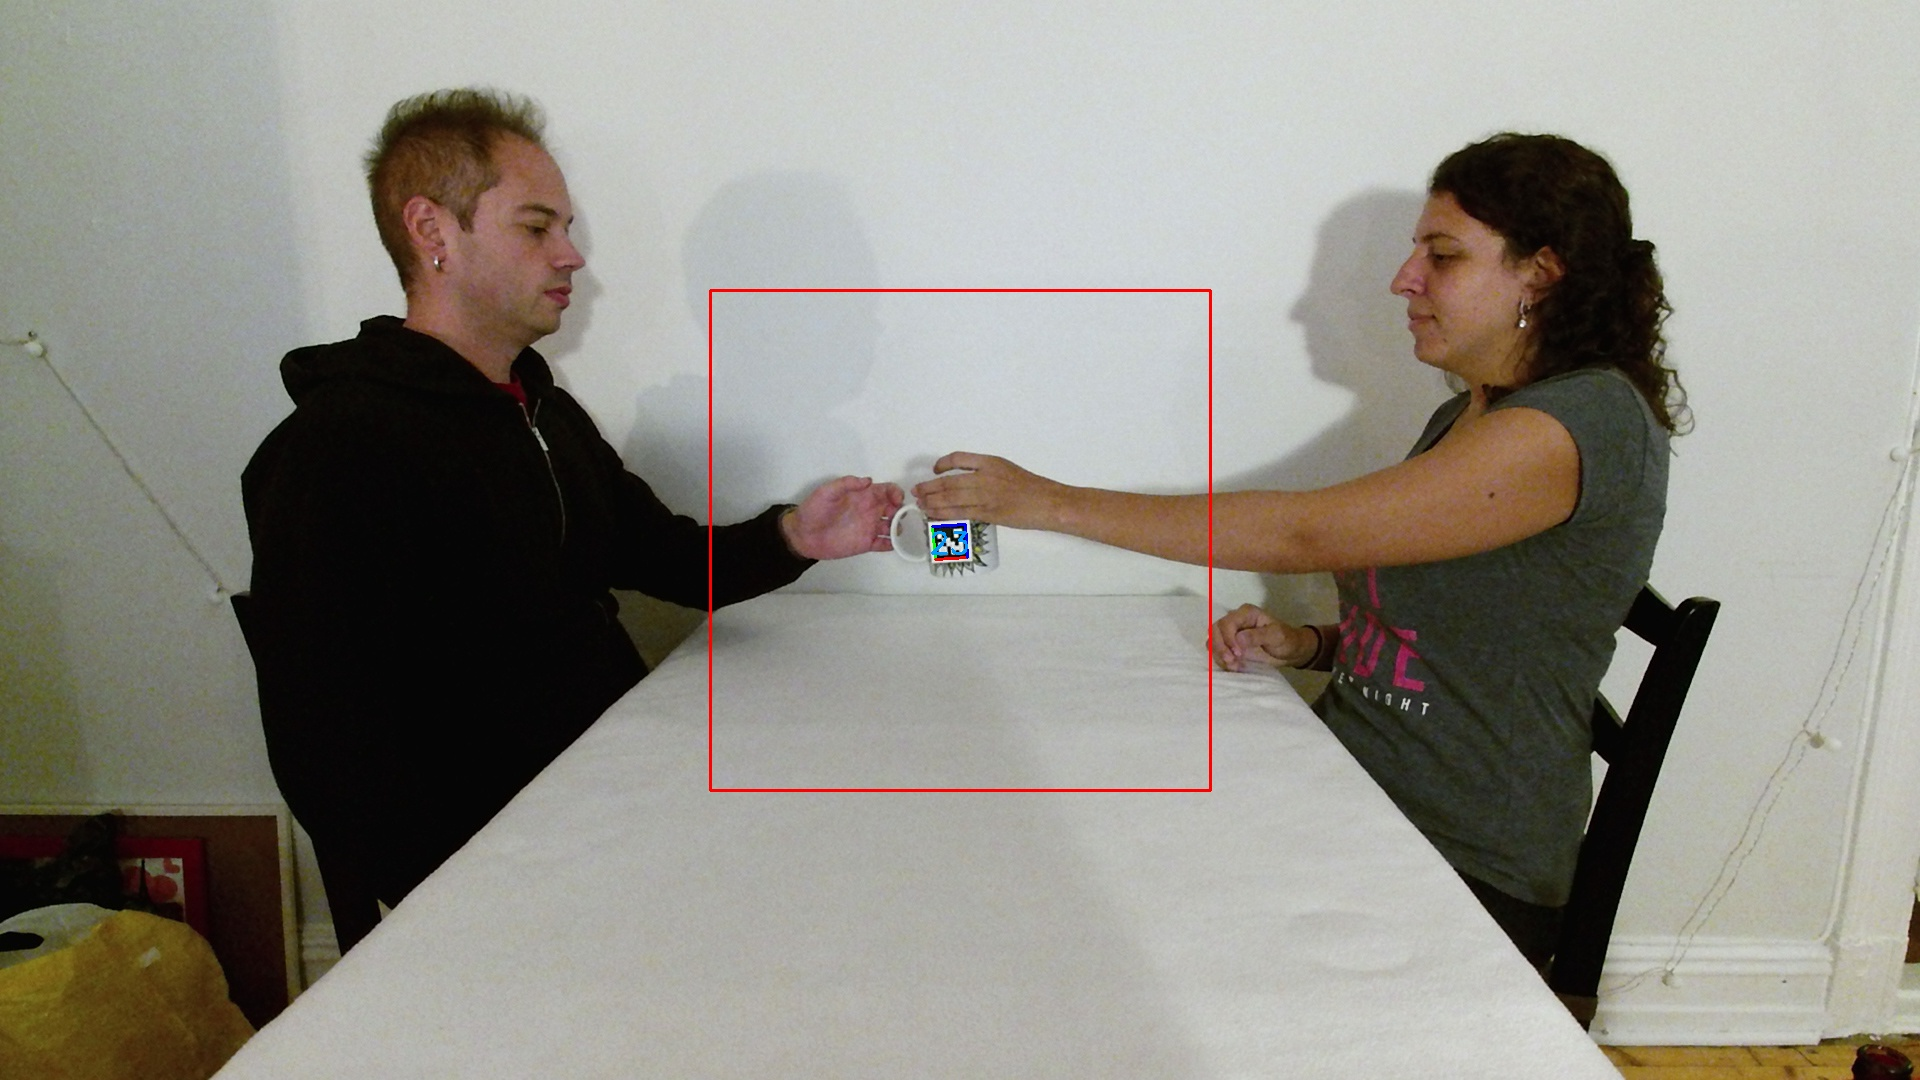
\includegraphics[width=\textwidth]{img/conclusion/awkward_handover_frame.jpg}
	\caption{Some grasps could become unnatural because of the AprilTags}
	\label{fig:fw_handover_awkward}
\end{figure}

Handover classes from clustering are however not enough to tell a robot how to grasp an object when handing it over. As seen in the results when the settings of one class are applied to an object the grasp region can become outside of it, though rotation and direction from center of object are correct. Future work would have to include calculating more precisely where a robot can grasp the object when handing it over given the data from the handover class.

Considering the amount of data that is needed for successfully training a CNN to perform object classification one can wonder if it is the best choice for such an application. In this work we needed to take help of pre-trained weights to classify the objects successfully, but without we get very poor accuracy. If trained from the scratch the system would need to observe quite many different objects to classify them correctly, also know when different objects are the same class. Future work would be to investigate results using other learning algorithms for images, or feature extraction from the objects and learn from them instead.
